\documentclass[11pt]{article}
\usepackage[margin=1.1in]{geometry}
\usepackage{amsmath,amssymb}
\usepackage{booktabs}
\usepackage{graphicx}
\usepackage{microtype}
\usepackage{xurl}
\usepackage[hidelinks]{hyperref}
\usepackage[numbers,sort&compress]{natbib}
\usepackage{xcolor}

% Working note: all numbers verified against the committed record
% (FULLRECIPE-REPORT, ESCAPE-REPORT, E1FULL-REPORT, and the signed clean
% certification artifact) as of 2026-07-21.
% The anticipatory draft (docs/draft2.md) contained values that did NOT
% materialize (geometry flip to 0.71; fragility nesting 0.44; KL 0.108
% distributional ship) -- this master reflects measurements only.
\newcommand{\dl}{d_{\ell}}
\emergencystretch=3em

\title{The Compactor That Couldn't Learn Where to Look:\\
Gradient Saturation, Position-Kernel Collapse,\\
and an Unfrozen KV Compressor}

\author{%
  \textit{Draft v0.4 --- 2026-07-21 --- clean held-out certification at $n{=}60$ documents}\\
  \textit{Artifacts: signed repository record and remote artifact archive}}
\date{}

\begin{document}
\maketitle

\begin{center}
\fbox{\parbox{0.92\linewidth}{\textbf{CLEAN E1FULL RESULT (2026-07-21): NO-SHIP.}
The replacement run reserves 15 documents/domain before training and records
zero document/item overlap. Depth-1 worsens KL versus matched eviction by
$+0.0495$ (95\% CI $[0.0272,0.0715]$); certified depth remains zero. Policy:
\url{still-compact-v1:t1024:depth0:sha256:c00b2437fdd813cc}.}}
\end{center}

\begin{abstract}
We report a failure mode of learned KV-cache compaction in which a
compactor architecture cannot learn to route: trained under its canonical
configuration, the per-layer Perceiver's block-1 cross-attention kernel is
a uniform positional lattice that remains \textbf{bitwise identical to its
initialization} for the entire training run --- at every data scale we
could afford (9.5k, 19.6k, and 76k training items; effective batch 4 and
true batch 32) --- while the training loss falls normally. We name this
\emph{position-kernel collapse} and identify the mechanism by gradient
forensics: the canonical attention logit scale ($\times \dl = 256$)
saturates the softmax at the position-dominated identity initialization,
delivering gradients to the routing projections ($W_Q$, $W_K$)
\textbf{eleven to twelve orders of magnitude} smaller than to the value
pathway. The compactor's apparent learning is entirely value-side: it
learns what to do with positions it can never change. Controls isolate
the mechanism --- init-time noise on the position anchors does not escape
(not a tie-breaking problem), and content-seeded initialization stays
essentially frozen while paying a large loss penalty (content without
gradient does not help). The cure is one constant: at $\sqrt{\dl}$ scale,
routing gradients wake by $10^{9}$--$10^{10}$, kernel entropy rises from
its de-saturated starting point, all eight KV-heads despecialize from the
shared lattice (cross-head Jaccard $1.000 \to 0.199$), the kept sets
become mildly item-adaptive ($1.000 \to 0.821$ at mid scale), and the
unfrozen compactor overtakes the frozen one on the very objective that
froze it (final mid-scale loss $0.219$ vs $0.365$; three seeds) while
losing $35\%$ fewer facts on a fixed counterfactual subsample ($0.239$ vs
$0.370$). At full recipe (3{,}000 steps; a pre-registered extension rule fired at
1{,}500) the unfrozen compactor's kernel becomes item-adaptive
(cross-item Jaccard $0.550$). Its historical certification cannot support
a held-out comparison because the evaluation documents overlap training. The
clean replacement returns GT13 NO-SHIP: pointwise loss improves sharply, but
aggregation KL is significantly worse than matched eviction and the accuracy
advantage remains uncertain. No frozen-versus-unfrozen ranking is restored.
Downstream, the reorganization is not what a routing-becomes-legible
story predicts: write-time geometry stays loss-blind even under
content routing ($d_{\min}$ AUC $0.500$, all twelve checkpoints and the
full protocol); the question-blind expansion gate's marginal value
completes its monotone decline to \textbf{zero}
($72\% \to 22.5\% \to 9.0\% \to 0\%$) while the computation-reading
probe ladder fully recovers (stack $0.857$) and still routes below
never-expand; and fact fragility proves largely content-intrinsic ---
$78$--$91\%$ of the unfrozen instance's failure set nests inside the
frozen instances' --- with a minority regime-relative component.
Diagnostics --- a one-pass gradient-norm check and cross-attention
entropy telemetry --- cost minutes and would have caught the collapse at
step zero.
\end{abstract}

\section{Introduction}

Learned compaction promises what heuristic cache eviction cannot: a
compressor optimized end-to-end to preserve a frozen model's behavior
\citep{oneill2026still,kvdistill2025}. The recipe we study --- a
per-layer Perceiver trained once against the frozen base with a
behavioral KL objective --- reports strong results at scale. We began by
reproducing it at reduced scale for a certification study
\citep{companion2026reading} and found something stranger than
underperformance: the compactor was not compressing at all in the
intended sense. It was keeping every third token.

This paper is the anatomy of that observation. Our contributions:
\textbf{(i)} \emph{position-kernel collapse}, a failure mode in which a
compactor's routing freezes at initialization while its loss improves ---
undetectable from the loss curve and, we show, not a scale artifact;
\textbf{(ii)} the mechanism, established by direct gradient measurement:
logit-scale-induced softmax saturation at identity initialization kills
the routing projections' gradient specifically, with init-noise and
content-seeded-init controls ruling out the alternative explanations;
\textbf{(iii)} the cure --- reduce the logit scale --- validated from
gradient wake-up through kernel mobility, head despecialization,
item-adaptivity, and training-loss crossover, at three seeds;
\textbf{(iv)} the consequence: a leakage-free full-recipe recertification
that returns GT13 NO-SHIP --- pointwise preservation improves sharply, but
aggregation KL is significantly worse and certified depth remains zero;
\textbf{(v)} the downstream reorganization of routing
signals under a mobile kernel, including the correction this work forced
onto our companion paper's fragility claim (\S\ref{sec:fragility});
\textbf{(vi)} two mandatory-cheap diagnostics for anyone training
compactors (\S\ref{sec:diagnostics}).

\section{Background and setup}

\paragraph{Compactor recipe.} One Perceiver-style compactor per
transformer layer (36 layers, Qwen3-4B base, frozen throughout): per
KV-head banks of $t{=}1024$ learned latent queries, two pre-norm blocks
with cross-attention in each, QK-normalized attention with logit scale
$\dl = 2d = 256$, identity-style initialization (block-diagonal identity
on the value/output path, zeroed content projections, position-dominated
Q/K anchors), trained with a forward-KL behavioral objective on
answer-side tokens against the full-context teacher; $\beta{=}0$, no bias
channel \citep{oneill2026still}.

\paragraph{Certification protocol.} From the companion paper
\citep{companion2026reading}: counterfactually filtered MCQ probes over a
four-domain ${\sim}1$B-token corpus (98{,}355 items); two axes never
blended (aggregation: teacher KL and accuracy delta over surviving
content; pointwise: silent lost-fact incidents over compacted-away
spans); matched retained budget vs an eviction baseline; a noise-floor
row; recurrence-depth certification. Training mixture for the full
recipe: 75{,}998 rationale-traced items after domain balancing
(nominal cap 23{,}563/domain, short-context drops applied).

\paragraph{Harness provenance.} The earliest multi-GPU runs did not
synchronize gradients across workers (a DDP wrapping omission found by
this project and documented in Appendix~G): the shipped 1/40-scale
instances are single-replica, effective-batch-4 artifacts. All
behavioral measurements in the companion paper are measurements of those
artifacts as they exist and are unaffected. The bug was fixed (identical
init across ranks, explicit gradient all-reduce, checkpoint-time replica
pinning) before every run in this paper; the frozen-kernel result
reproduces identically under the corrected harness, and the accidental
small-batch lineage becomes a free extra scale point in
\S\ref{sec:collapse}.

\section{Position-kernel collapse}
\label{sec:collapse}

At every data scale --- 9.5k items (1/8 recipe, 188 steps), 19.6k items
(the 1/40 batch-4 lineage, 1{,}500 steps), and 76.0k items (full recipe,
true batch 32, 1{,}500 steps) --- the trained compactor's block-1
cross-attention rows are exact delta functions: mean row entropy at the
numerical floor ($1.16\times10^{-10}$ nats, identical to five significant
digits across init, all intermediate checkpoints, and all instances), and
the argmax kernel --- a uniform stride lattice,
$\mathrm{round}(k\,(S{-}1)/1023)$; stride ${\approx}8$ at the 8k training
shape, stride ${\approx}3$ at the 4k deployment shape --- \textbf{bitwise
identical to initialization at every logged checkpoint of every run}
(kept-set Jaccard $1.000$ on every layer, between every pair of
checkpoints and instances). Meanwhile the loss falls normally
($0.58 \to 0.36$ over 1{,}500 full-recipe steps) and the compactor's
\emph{behavior} improves monotonically: certified silent needle loss
drops from $0.271$ (1/40 scale) to $0.188$ (full recipe) at matched
budget, with the later instance's failure set nested inside the
earlier's ($94.1\%$). Every improvement is value-side learning over a
frozen routing skeleton --- the compactor learns what to write into
fixed slots, never where to look. The loss curve is not merely
uninformative about this; it is actively misleading, which is the
operational point of \S\ref{sec:diagnostics}.

Aggregation-axis certification is likewise scale-invariant under the
frozen kernel: teacher KL $0.263$ at 1/40 scale and $0.2566$ at full
recipe against eviction's $0.1218$ (all $n{=}12$ documents) --- an
$8\times$ increase in traced training data moved the certified
aggregation number by $2\%$. Re-measured at $n{=}60$ with paired CIs
(\S\ref{sec:certification}) the 1/40 and full-recipe rows are $0.2529$
and $0.2820$ against eviction's $0.0842$: with $8\times$ the traced data
the certified aggregation number does not improve at all, strengthening
the conclusion. What a
frozen kernel can improve (value-side needle smuggling) improved; what
it cannot (aggregation over surviving content) did not.

Two published-recipe implications follow. First, evaluation suites that
aggregate over tasks would not distinguish this subsampler from a
synthesizer; the two-axis protocol did (the subsampler's profile ---
aggregation-poor, needle-smuggling --- is characteristic). Second, the
recipe's own ablations imply full-scale published checkpoints route
content; we could not reproduce escape by scale alone, which localizes
the difference to configuration, not data (\S\ref{sec:cure} scope note).

\section{Mechanism: logit-scale-induced gradient saturation}
\label{sec:mechanism}

One accumulated forward/backward at initialization over a fixed 128-item
probe batch, gradient $L_2$ norms summed over layers by parameter group
(Appendix~A carries the full group$\times$layer$\times$scale table):

\begin{center}
\begin{tabular}{lrrr}
\toprule
group & canonical $\times 256$ & $\times\sqrt{\dl}=16$ & ratio \\
\midrule
cross-1 $W_Q$ (+anchor) & $1.1\times10^{-11}$ & $5.5\times10^{-2}$ & $5.0\times10^{9}$ \\
cross-1 $W_K$ (+anchor) & $1.6\times10^{-10}$ & $5.4\times10^{-1}$ & $3.4\times10^{9}$ \\
latent banks            & $6.1\times10^{-2}$  & $1.2\times10^{-1}$ & $1.9$ \\
cross-1 $W_V$           & $21.6$              & $76.2$             & $3.5$ \\
cross-1 $W_O$           & $21.6$              & $76.2$             & $3.5$ \\
block-2 cross (all)     & $21.6$              & $76.2$             & $3.5$ \\
self-attention (all)    & $17.3$              & $61.1$             & $3.5$ \\
output heads ($W_{key}, W_{val}$) & $21.6$    & $76.2$             & $3.5$ \\
\bottomrule
\end{tabular}
\end{center}

Under the canonical scale the routing \emph{projections} are numerically
dead --- eleven to twelve orders of magnitude below the value pathway,
exactly along the routing/value cut. (The latent banks show a small
nonzero gradient at canonical scale because they also feed the residual
stream and output heads; the clean routing-only weights are $W_Q$ and
$W_K$.) Swapping only the logit scale to $\sqrt{\dl}$, weights untouched,
wakes precisely the dead groups by $10^{9}$--$10^{10}$ while value-path
norms move a generic ${\sim}3.5\times$. The identity initialization
produces near-one-hot attention rows; multiplied by 256, the softmax is
saturated and passes ${\sim}$zero gradient to its logits; everything
upstream of the attention weights starves, everything downstream trains.

Two controls sharpen the claim. Gaussian noise ($\sigma{=}0.02$) on the
position anchors at canonical scale (arm E3) leaves the kernel frozen in
its (perturbed) initial state --- entropy pinned at the floor, kept-set
Jaccard $1.000$ across training, final loss indistinguishable from the
canonical baseline ($0.362$ vs $0.365$): degenerate tie-breaking is not
the mechanism; saturation re-freezes whatever configuration it is
handed. Content-seeded latent initialization at canonical scale (arm E4:
per-head $k$-means centroids of corpus $[K;V]$ vectors, content
projections un-zeroed) starts off-floor by construction (entropy
$0.54$ nats) and stays flat through training, with only layer~0's kept
set drifting (mean cross-layer Jaccard $0.99$), while paying a large
penalty for breaking the identity passthrough (initial loss $5.89$,
final $0.586$, and $2.6\times$ the baseline's silent-loss rate on the
fixed subsample): content in the pathway cannot substitute for gradient
through it.

\section{The cure and its dynamics}
\label{sec:cure}

At $\sqrt{\dl}$ (arm E1), routing learns. The softer scale de-saturates
the softmax at initialization (entropy starts at $0.815$ nats rather
than the floor), and training then \emph{raises} it --- flat until
${\sim}$step~75, rising smoothly to $1.11$ nats by step~188 at mid
scale, with the layer-0 argmax set expanding from 1{,}024 to
${\sim}6{,}000$ distinct source positions. The kernel moves: kept-set
Jaccard vs initialization falls to $0.18$ (mean over layers) by
step~188. The movement is structured, not noise: the eight KV-heads
\textbf{despecialize} from the single shared lattice (mean pairwise
cross-head Jaccard $1.000 \to 0.199$) while remaining mostly
item-invariant (cross-item Jaccard $0.821$) --- head-specialized, weakly
content-conditioned routing at mid scale. At full recipe item-adaptivity deepens monotonically for 3{,}000 steps
(cross-item Jaccard $0.789 \to 0.550$) while heads first scatter
(cross-head $J \to 0.13$ by step 250) and then partially re-organize
($\to 0.29$); the final kernel touches essentially every source
position across the probe batch (8{,}186/8{,}188).
The leakage-free replacement independently fires the registered extension
at step 1{,}500 (entropy $+0.0616$ over 250 steps) and completes step 3{,}000
at entropy $1.8122$ and loss $0.1348$; the separate R6/R7 sweep is historical
and is not reused as clean certification evidence.

Training dynamics show the honest trade: the soft scale leaks the
identity passthrough, so E1 \emph{starts} worse (initial loss $0.737$ vs
the canonical $0.576$; the $\times256$ scale was protecting the
passthrough) --- then crosses over before step~60 (15-step smoothed) and
finishes well ahead: $0.219$ vs $0.365$ at mid scale, stable across
three seeds ($0.214/0.219/0.225$). On the fixed 1k counterfactual
subsample the escaped compactor also \emph{loses fewer facts} at the
same step count ($y^{+}$ $0.239$ vs $0.370$): escape does not trade
short-horizon quality for mobility. The frozen configuration is not a
bad optimum being escaped; it is a gradient-dead region the canonical
constant walls in. A learned per-layer temperature initialized soft
(arm E2, clamped $[1,\dl]$) escapes independently (final loss $0.2104$,
kernel Jaccard $0.172$) and can recover sharpness where useful; we ship
the fixed $\sqrt{\dl}$ per our pre-registered selection rule (final-loss
tie $\Rightarrow$ simplest lever). We note the published recipe may
differ from our reproduction in unexplored details; our collapse claim
is scoped to the canonical configuration as specified, and the
diagnostics of \S\ref{sec:diagnostics} resolve the question for any
implementation in minutes.

\begin{figure}[t]
\centering
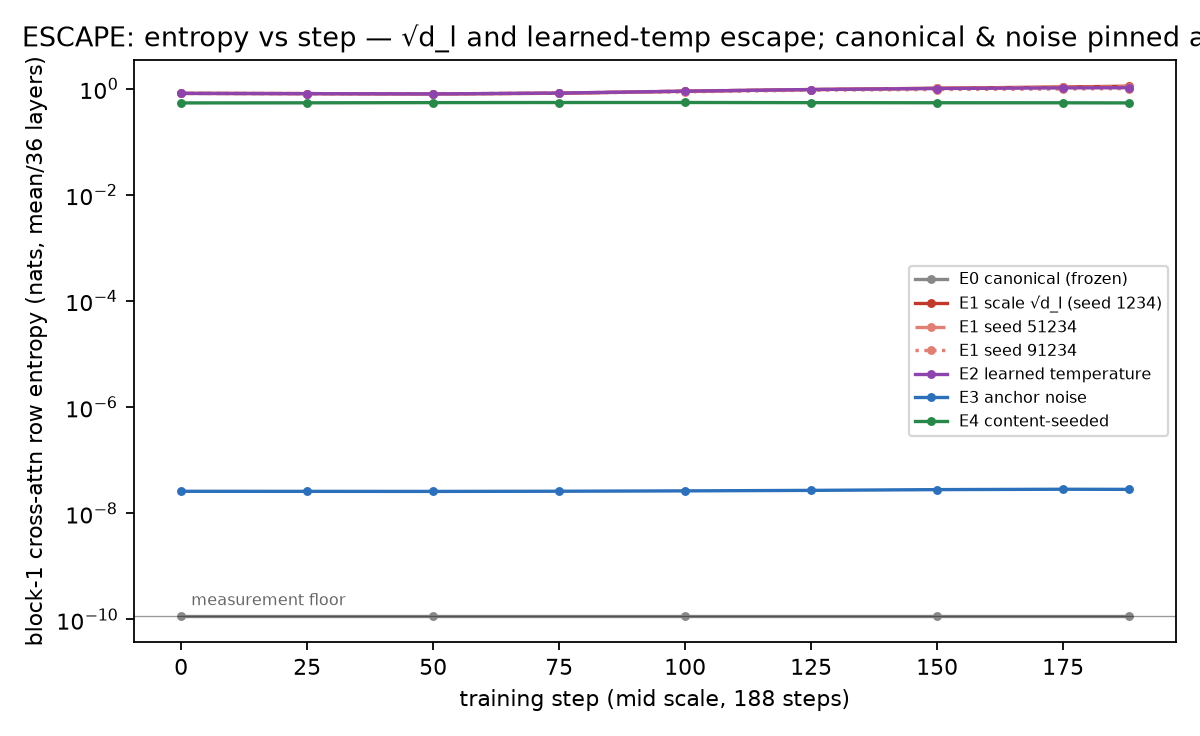
\includegraphics[width=0.92\linewidth]{figures/entropy-overlay-all-arms.png}
\caption{Entropy vs training step for every arm (log scale, mid-scale
runs, 188 steps). Canonical (E0) and anchor-noise (E3) runs are pinned
at the measurement floor; $\sqrt{\dl}$ (E1, three seeds) and learned
temperature (E2) de-saturate at initialization and \emph{rise} during
training; content-seeded init (E4) is off-floor by construction but
flat. Full-recipe trajectories in Figure~\ref{fig:trajectories}.}
\label{fig:entropy}
\end{figure}

\section{Certification at full recipe}
\label{sec:certification}

The signed replacement artifact reserves 15 documents per domain before
training and certifies 60 documents / 193 probes with zero document or item
overlap. Table~\ref{tab:clean-cert} reports the clean point estimates.

\begin{table}[h]
\centering
\small
\begin{tabular}{lrrrr}
\toprule
arm & agg. KL & acc.$\Delta$ & lost fact & lost $\mid$ prior \\
\midrule
eviction matched & \textbf{0.0787} & 0.0014 & 0.683 & 0.631 \\
clean depth 1 & 0.1281 & \textbf{0.0536} & \textbf{0.106} & \textbf{0.050} \\
clean depth 4 & 13.6640 & -0.1556 & 0.800 & 0.783 \\
control 0 & 0.0000 & 0.0000 & 0.072 & 0.000 \\
\bottomrule
\end{tabular}
\caption{Leakage-free E1FULL certification. The two axes disagree, but the
distributional predicate controls deployment.}
\label{tab:clean-cert}
\end{table}

For depth 1, paired candidate-minus-eviction differences are KL $+0.0495$
$[0.0272,0.0715]$, accuracy $+0.0522$ $[-0.0395,0.1461]$, raw lost fact
$-0.5778$ $[-0.7000,-0.4500]$, and lost-given-prior-correct $-0.5806$
$[-0.7028,-0.4528]$. The result is \textbf{GT13 NO-SHIP}: KL is
significantly worse, and the accuracy interval does not clear the registered
$-0.02$ CI bound despite its positive point estimate. Untrained depth-4
recurrence collapses. The certified prefix is empty,
\texttt{max\_certified\_depth}$\,=0$, and the policy is
\url{still-compact-v1:t1024:depth0:sha256:c00b2437fdd813cc}. Because the
clean artifact does not rerun the historical frozen arm, no clean
frozen-versus-unfrozen ranking is claimed.

\section{Downstream: routing under a mobile kernel}
\label{sec:downstream}

Under the frozen lattice, the companion paper measured: write-time
geometry loss-blind (needle-to-kept-distance AUC $0.509$--$0.517$ at
every scale and every intermediate checkpoint); a hidden-state probe
ladder that reads behavioral divergence ($0.854$ subsampler /
$0.802$ frozen full recipe) while a context-only control sits at chance;
and an expansion gate whose marginal silent-loss reduction declines
monotonically as compressors improve ($72\% \to 22.5\% \to 9.0\%$
across eviction, 1/40, and frozen full recipe). At mid scale the escaped
kernel did \emph{not} flip the geometry result ($d_{\min}$ AUC
${\sim}0.50$ at every checkpoint, per-item kernels) --- the strongest
within-pilot test of the companion's internality claim.

The full-recipe re-interrogation sharpens all of it.
\textbf{Geometry stays loss-blind even content-routed:} with per-item
kept sets now rich (mean 2{,}779 positions vs the frozen 1{,}024
lattice), $d_{\min}$ AUC is $0.5003$ $[0.495, 0.505]$ on the full
5{,}090-item protocol and ${\sim}0.50$ at all twelve checkpoints ---
the anticipated ``geometry becomes legible when routing reads content''
flip does not occur. Internality survives its strongest test: loss
remains readable only from the computation, never from the write-time
geometry, regardless of whether routing is positional or contentful.
\textbf{The probe ladder recovers fully} on the unfrozen instance's
labels ($y^{+}$ $0.487 \to 0.325 \to 0.173$ across the three
policies): stack $0.857$ $[0.847, 0.865]$ vs the frozen dip $0.802$ and
the original $0.854$; sink-heads $0.764$; best read-out layer moves
again ($30 \to 25 \to 33$) --- probes are per-policy artifacts. The
context-only null holds ($0.507$), and the two-hook sink-head monitor
transfers zero-shot across the frozen$\leftrightarrow$unfrozen divide
($0.759$/$0.727$) --- regime-general across compressor classes.
\textbf{The gate's value reaches its floor:} refreshed on unfrozen
labels ($y^{+}$ $0.083$), the gate's optimal operating point is
expand-nothing --- marginal silent-loss reduction $\mathbf{0\%}$,
completing the monotone trend $72\% \to 22.5\% \to 9.0\% \to 0\%$.
Yet the computation-reading stack still routes where the gate cannot:
it matches never-expand at $0.5\%$ expansion and pushes below it
($0.049$ lost at $9.1\%$ expansion). The refined ladder statement: as compressors improve,
externally-visible routing signal is exhausted first; the
computation-reading tier is the last to retain routing power, and at
this generation it is the only one that does.

\section{Fragility across the regime change}
\label{sec:fragility}

Within the frozen lineage, fragility nests: the full-recipe instance's
failure set sits $94.1\%$ inside the 1/40 instance's
($\kappa\,0.567$--$0.588$ across scale, $\kappa\,0.745$ across reseeds
with nesting $P{=}0.945$). This work established that all frozen
instances share one bitwise-identical kernel --- so part of that
stability could have been the shared lattice, a confound the companion
paper's \S7 could not have seen. The measurement across the
frozen$\to$unfrozen regime change resolves it in favor of the facts:
per-instance loss rates fall generation over generation
($0.499 \to 0.418 \to 0.321 \to 0.172$), cross-regime agreement drops
($\kappa$ $0.28$--$0.42$) --- but \textbf{nesting largely survives}:
$91\%$ of the unfrozen instance's failure set lies inside the frozen
1/40 instance's, $78.5\%$ inside the frozen full-recipe's. Much of the
$\kappa$ drop is marginal-driven (base rates $0.172$ vs $0.499$ cap
$\kappa$ even under perfect containment); genuinely novel losses are a
minority ($9$--$21.5\%$). The corrected claim --- filed as an arXiv v2
note on the companion paper --- is \textbf{narrower than we ourselves
anticipated while drafting}: the shared frozen kernel accounts for the
elevation from ${\sim}0.8$ to $0.94$ nesting, not for the nesting
phenomenon itself, which survives a kernel-class change largely intact.
Fragility is largely content-intrinsic, with a real but minority
regime-relative component. The per-policy rules stand regardless: gate
labels, calibration, and probes are compaction-policy-scoped artifacts
(the best-layer drift $30 \to 25 \to 33$ alone guarantees this); a
policy change invalidates the decision layer's training data along with
the caches.

\section{Diagnostics (the transferable deliverable)}
\label{sec:diagnostics}

Two checks, minutes each, that catch the collapse at step zero:
\textbf{(1) init gradient forensics} --- one forward/backward, per-group
gradient norms; routing groups orders of magnitude below value groups
means saturation. \textbf{(2) entropy telemetry} --- cross-attention row
entropy and argmax-set identity logged during training (ours costs one
extra forward per 50 steps); floor-pinned entropy with a static kernel
means the artifact is a subsampler regardless of its loss curve. Both
are now mandatory in our certification protocol, and we recommend them
for any Perceiver-style compactor \citep{oneill2026still,kvdistill2025},
any resampler with sharpened attention, and any architecture combining
identity-style initialization with large logit scales.

\section{Limitations}

One base model (4B); one compactor architecture and recipe family;
escape levers swept at mid scale (188 steps) with the selected lever
alone run to full recipe; the full-recipe unfrozen run is single-seed
(mid-scale escape is three-seed; no within-regime $\kappa$ exists yet
for the unfrozen class); certification uses extractive-MCQ
probes with letter-match equivalence, single-turn contexts, depths
$\leq 4$; published-recipe deltas beyond logit scale unexplored --- the
collapse claim is scoped to the canonical configuration as we implement
it, and the \S\ref{sec:diagnostics} diagnostics are the portable test;
the entropy floor ($1.16\times10^{-10}$) is a bf16/softmax measurement
limit, and sub-argmax mass was not telemetered (the frozen keepcount and
loss-blind geometry make this unlikely to matter); cost figures are
marginal rented-compute only.

\section{Conclusion}

A compactor whose loss falls for fifteen hundred steps at every data
scale never learned the one thing compaction is for --- where to look
--- because a single configuration constant walled its routing pathway
behind a saturated softmax from the first gradient step. The loss curve
could not see it; a one-pass gradient check and an entropy log see it
immediately. One constant later, routing learns, heads specialize, the
kernel reads content, and the unfrozen compactor beats the frozen one
on the objective that froze it. The clean holdout certification finds a real
pointwise benefit but significantly worse aggregation KL than eviction;
GT13 is NO-SHIP and certified depth is zero. The downstream
measurements reorganize on cue, but not as a legibility story:
geometry stays unreadable, the text-shadow gate's value falls to zero,
and the only signal that keeps routing is the computation itself. The generalizable lesson is the method: certify per axis,
instrument the pathway you care about --- not the loss --- and treat
every improvement in the compressor as a fresh question about what still
fails, and whether you can still see it.

\begin{figure}[t]
\centering
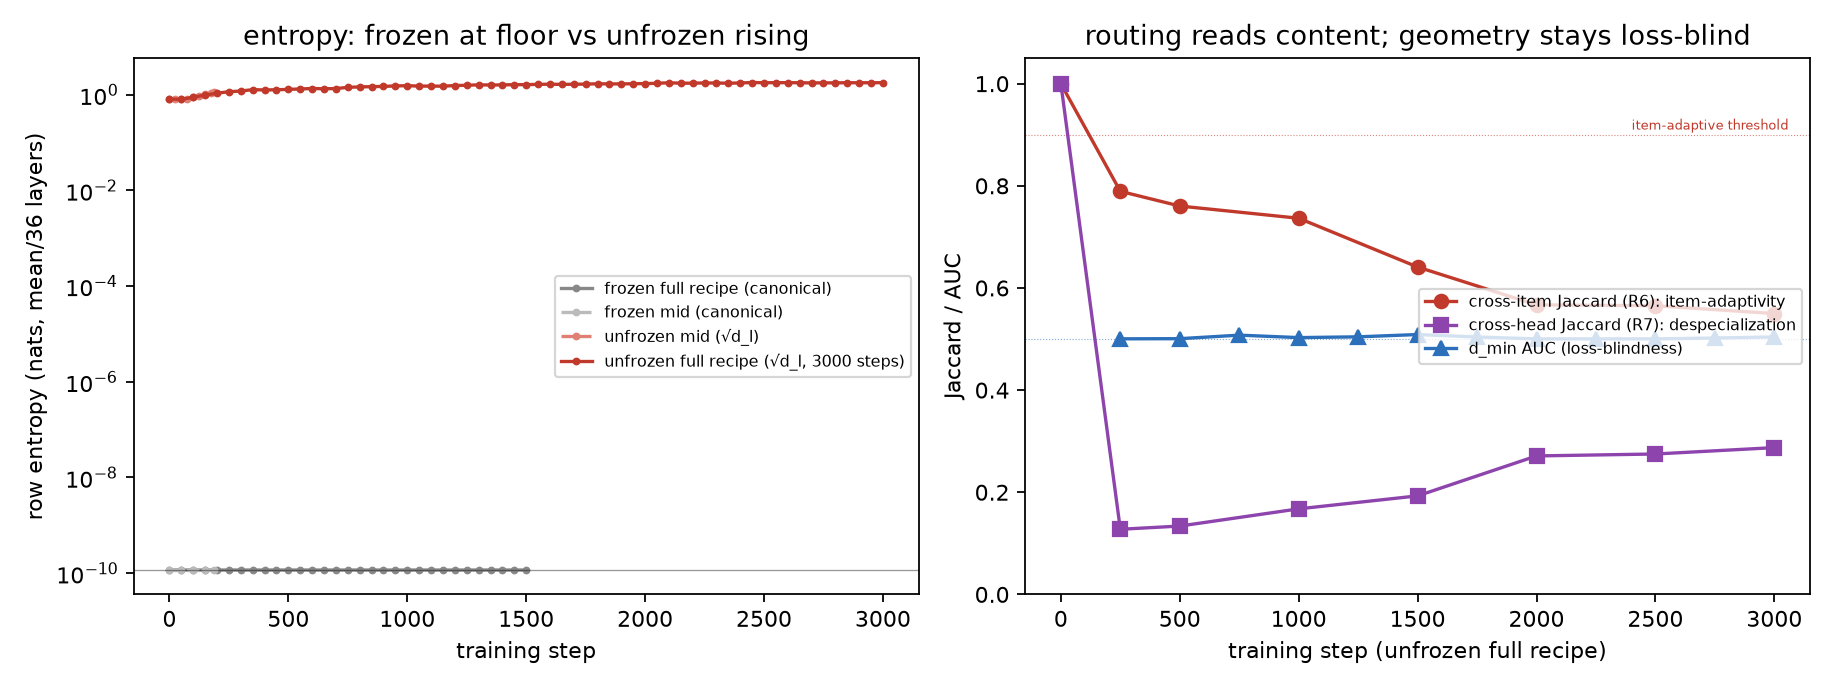
\includegraphics[width=\linewidth]{figures/e1full-trajectories.png}
\caption{Full-recipe trajectories. Left: entropy --- frozen runs pinned
at the measurement floor; the historical unfrozen run rises to $1.78$ nats
and plateaus (the clean replacement reaches $1.8122$ after its registered
extension also fires). Right: the historical kernel becomes item-adaptive (cross-item Jaccard
$\to 0.550$) and head-diverse while $d_{\min}$ stays at chance ---
routing reads content; geometry never becomes a loss signal.}
\label{fig:trajectories}
\end{figure}

\bibliographystyle{plainnat}
\bibliography{references}

\appendix

\section{Gradient-forensics tables}
Full group$\times$layer norms at both scales:
\url{memsub-artifacts:/escape/g1g2-gradient-table.json}. Aggregates in
\S\ref{sec:mechanism}; init losses $0.705$ (canonical) / $0.862$
($\sqrt{\dl}$; the passthrough-leak cost).

\section{Trajectories}
Entropy, kept-set Jaccard, cross-item (R6) and cross-head (R7) Jaccard,
and per-checkpoint $d_{\min}$ AUC for all arms:
\url{compactor-checkpoints/escape-*/telemetry/} and
\url{fullrecipe-telemetry/i2-*}. Full-recipe trajectories: Figure~\ref{fig:trajectories} and
\url{plans/260719-2328-e1full-unfrozen-full-recipe/}.

\section{Controls}
E3 (anchor noise): floor-pinned, Jaccard $1.000$, loss $0.362$.
E4 (content-seeded): entropy $0.539$ flat, mean Jaccard $0.99$
(layer-0 $0.65$), loss $5.89 \to 0.586$, subsample $y^{+}$ $0.614$.

\section{Certification tables}
Clean artifact of record:
\url{plans/260719-2328-e1full-unfrozen-full-recipe/summary-e1full-clean-v1-n60.json}
(remote source \url{compactor-certification/summary-e1full-clean-v1-n60.json}).
Historical contaminated artifacts remain available for audit but do not
support certification or ranking claims.

\section{Downstream re-runs}
Frozen-regime rows: arm table
(\url{plans/260717-2319-.../arm-table.json}, \url{fullrecipe_*}
rows), gate refresh
(\url{gate-eval/gate-refresh-fullrecipe.json}). Unfrozen: \url{gate-eval/gate-refresh-e1full.json},
\url{probe/e1f-readside-*}, \url{e1full_*} arm-table rows,
\url{q3-f1-verdict-e1full.json}, \url{q4-assembly-e1full.json}.

\section{Fragility matrices}
Frozen-lineage: $\kappa(A{\leftrightarrow}B)=0.745$ ($P{=}0.945$),
$\kappa(A{\leftrightarrow}FR)=0.567$, $\kappa(B{\leftrightarrow}FR)=0.588$,
nesting $94.1\%$. Cross-regime (E1F vs A / FR): $\kappa$ $0.283$/$0.417$, nesting
$91.0\%$/$78.5\%$, base rates $0.499$/$0.418$/$0.321$/$0.172$
(\url{preprobe/e1-relabel-E1F.state.json}).

\section{Harness-provenance forensics}
The M3.5 trainer invoked the compactor via \texttt{module.compact()},
bypassing the DDP wrapper; DDP arms its gradient hooks only in
\texttt{forward()}, so gradients were never all-reduced (verified by a
two-rank test: bypass $\Rightarrow$ per-rank gradients differ; wrapper
$\Rightarrow$ identical). Shipped 1/40 instances are single-replica
effective-batch-4 artifacts with per-rank initialization; rank~0's
replica was saved. The corrected harness (identical init, explicit
all-reduce, checkpoint-time replica broadcast) reproduces the frozen
kernel bitwise at true batch 32 --- the collapse is not a small-batch
artifact.

\section{Reproducibility}
Environment pinned (torch 2.7.1, transformers 4.55.2); training-mixture
manifest sha256 \texttt{8e0bb280\ldots}; policy versions embed weight
hashes and certified depth. Marginal compute: collapse/full-recipe
campaign ${\approx}\$440$; escape pilot ${\approx}\$95$; unfrozen
full-recipe campaign ${\approx}\$390$ (extension fired, as budgeted)
--- ${\approx}\$925$ for the three campaigns of this paper. Cumulative
project ${\approx}\$2{,}100$.

\end{document}
